\section{Dynamic programming}

There are two main ways to increase the efficiency of an algorithm:
``don't do anything twice'' and ``don't do anything stupid''.
While the definition of stupid is not obvious and
``not being stupid'' is quite difficult,
``don't do anything twice'' is quite clear and fixing your algorithm
with it is quite easy. That's what DP is about.

\subsection{Example 1: Fibonacci sequence}
We use the Fibonacci sequence as a first example to introduce Dynamic Programming. 

We want to find the $n$-th Fibonacci number.
If we just implement the definition of the Fibonacci sequence, we get:
\begin{verbatim}
int fibo(int n)
{
    if(n==0)
        return 0;
    else if(n==1)
        return 1;
    else
        return fibo(n-1) + fibo(n-2);
}
\end{verbatim}
However, since \texttt{fibo(n)} calls both \texttt{fibo(n-1)} and
\texttt{fibo(n-2)}, the running time of that function will about double
every time $n$ increases by 1.
So the complexity is $O(2^n)$, which is quite crappy.\footnote{Actually, it's more like $O(\phi^n)$, but this doesn't affect the crappiness.}
That's because we compute the same thing \emph{many} times.
To avoid that, we just have to remember the solutions to the sub-problems,
that is, the previous Fibonacci numbers, in an array.
Then we can just fill up the array progressively, which only takes $n$ steps.
\begin{verbatim}
int fibo(int n)
{
    vector<int> f;
    f.push_back(0);
    f.push_back(1);
    for(int i=2; i<=n; i++)
        f.push_back(f[i-1] + f[i-2]);
    return f[n];
}
\end{verbatim}

We actually only need the last two Fibonacci numbers in every iteration, so we can even improve the space complexity from $O(n)$ to $O(1)$.
Note that for this particular problem, even better algorithms exist. We only show this version to illustrate dynamic programming.



\subsection{Example 2: Longest increasing subsequence}

However, finding which sub-problems to solve is not always as easy,
as the second example shows.

In the longest increasing subsequence problem, you have to find the longest
increasing sequence of (not necessarily consecutive) elements in an array of length $n$.
For example, in the list $[4,7,5,1,3,2,6,8]$, longest increasing subsequences
would be $[4,5,6,8]$ or $[1,2,6,8]$. (The solution is not unique.)

Trying all subsequences and finding the longest increasing one would
take $O(2^n)$ time, as every number in the array may or may not be in
the subsequence.


A first intuition might be to start from the beginning and keep the longest
increasing subsequence so far in memory, and add to it as we go.
But the problem is that it might not find the best solution.
In $[4,7,5,1,3,2,6,8]$, for example, it will add 4, then 7, but then
it will not add any element until 8, giving $[4,7,8]$, which is not optimal.

\subsubsection{Naive recursive implementation}
Another idea might be to recursively find the longest increasing subsequence which can be concatenated to a prefix of the array.
This naive (recursive) implementation is shown in Listing~\ref{code-lis1}.
\lstinputlisting[label=code-lis1,caption=Naive recursive implementation, language=C++,firstline=4, lastline=17, tabsize=2, breaklines=true, numbers=left, float]{src/lis/naive.cpp}
However, this algorithm has a very bad time complexity.

\subsubsection{Store maximal sequence length for a certain ending value}
Actually, when we want to add some element $a[i]$ of the array $a$,
instead of trying to add it to the longest increasing subsequence
between $0$ and $i-1$, we can try to find the longest
increasing subsequence that ends with an element smaller than $a[i]$.
So we could keep a table of the longest increasing subsequences
ending with all possible values.
A possible implementation is shown in Listing~\ref{code-lis2}.
\lstinputlisting[label=code-lis2,caption=Storing maximal sequence length for a certain ending value, language=C++,firstline=6, lastline=38, tabsize=2, breaklines=true, numbers=left, float]{src/lis/victor.cpp}
Beware: this assumes that the max value in array $a$ is smaller than $n$
(we could remap the values if this is not the case).
The time complexity is $O(n^2)$, much better than $O(2^n)$,
but we can still do better (and more convenient).

\subsubsection{Store smallest ending value index for a certain sequence length}
Instead of looking at the longest subsequence for some value,
let us do the opposite
and look at the smallest ending value for which there is a subsequence
of some length.
We would then have to find the biggest length such that the ending value
is smaller than the current element.

Let's name this array \texttt{smallest\_end\_for[]}.
It will contain the \emph{index} of the smallest ending value.
If you can achieve some length with an element, then you can achieve
any shorter length, so \texttt{smallest\_end\_for} is non-decreasing.
So you can just use binary search to find the longest subsequence
there is ending with an element smaller than $a[i]$. Let's say its length is
\texttt{prev\_len}.

Then you just have to update \texttt{smallest\_end\_for[prev\_len+1]}
if the solution you've just found is better than the previous one.
You don't have to update anything else, since the lengths 1 to
\texttt{prev\_len}
can already end with smaller values.
The implementation is shown in Listing~\ref{code-lis3}.

\lstinputlisting[label=code-lis3,caption=Storing smallest ending value index for a certain sequence length, language=C++,firstline=6, lastline=38, tabsize=2, breaklines=true, numbers=left, float]{src/lis/victor.cpp}

Since the outer loop is run $n$ times and the inner loop is run
at most $\log_2 n$ times, the total complexity is $O(n\log n)$.

Note: both algorithms can be adapted to output the generated
subsequence as well, not just its length.

\subsection{Approaches}
\subsubsection{Bottom-up}
The previous examples showed how you can use dynamic programming to build up a solution to a problem based on previously calculated smaller sub-problems.
The algorithms first calculated the solutions to all smaller sub-problems, always using the previously calculated solutions to their predecessors.
This approach is called \emph{bottom-up}.

\subsubsection{Top-down}
Another approach to dynamic programming consist of caching results whenever they are calculated. 
Instead of first calculating the solutions to all smaller problems, we now wait to calculate them until we need them.
As soon as we have calculated them, they are stored in a caching table. 
Whenever the algorithm needs the same solution, it can find it in the caching table instead of recalculating it.
\subsection{2-dimensional DP}
We illustrate the two approaches using a simple grid problem.

You are asked to find the minimal-cost path from the top-left corner to the bottom-right corner of the grid.
You can only walk right and down to adjacent tiles. The cost of the path equals the sum of the values of the tiles you walk through.

It is easy to see that the cost to reach a tile is equal to the value of the tile plus the cost to reach the tile on top of it or plus the cost to reach the tile left of it.
Figure~\ref{image:2d-problem} show the problem. Figure~\ref{image:2d-solution} shows for every tile the cost to get there.

\begin{figure}
\label{image:2d-problem}
 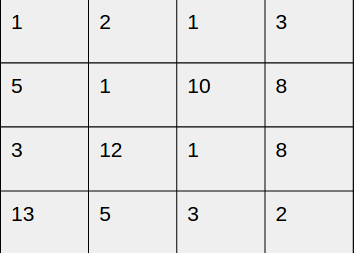
\includegraphics{2d/problem.png}
 \caption{The grid with on each tile the cost to walk through it.}
\end{figure}
\begin{figure}
  \label{image:2d-solution}
 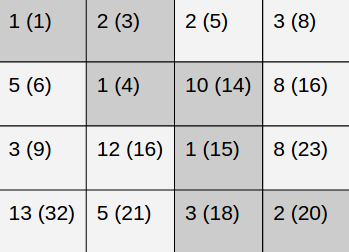
\includegraphics{2d/solution.png}
 \caption{The grid with on each tile the cost to walk through it and between brackets the cheapest way to get there (cost to walk throught the tile itself included).}
\end{figure}

The first algorithm shows the top-down approach. 
Whenever we need the cost to reach a certain tile, it checks whether the cost has been calculated.
If this is not the case, it calculates the solution for this tile.
If the cost was calculated earlier, it just uses the previously calculated value.
The code is shown in Listing~\ref{code-2d-1}.
\lstinputlisting[label=code-2d-1,caption=Top-down approach, language=C++,firstline=8, lastline=20, tabsize=2, breaklines=true, numbers=left, float]{src/2d/topdown.cpp}

The second algorithm shows the bottom-up approach.
We first populate the top row and left column of the table. 
Next, the algorithm fills all elements in the table row per row from left to right.
In this step, it uses the values of the tile on top of the current tile and the tile left of the current tile.
The code is shown in Listing~\ref{code-2d-2}.
\lstinputlisting[label=code-2d-2,caption=Bottom-up approach, language=C++,firstline=8, lastline=18, tabsize=2, breaklines=true, numbers=left, float]{src/2d/bottomup.cpp}
\subsection{Recognizing dynamic programming problems}
Typical problems involving a dynamic programming solution include:
\begin{enumerate}
 \item Sequences
 \begin{enumerate}
  \item Longest increasing subsequence
  \item Longest common substring
  \item Recursive definitions of a series of number (e.g. Fibonacci)
 \end{enumerate}
 \item Knapsack (Given a backpack of capacity C and a set S of items with a given size $s_i$ and value $v_i$, choose a subset of S that fits in the backpack, maximizing the total value.)
 \item 'Divide and Conquer' algorithms with overlapping sub-problems.
\end{enumerate}

\subsection{Applications}
The Dynamic Programming technique is used in various well-known algorithms, such as:
\begin{enumerate}
 \item Bellman-Ford algorithm (Single-source shortest path that can handle negative edge weights)
 \item Floy-Warshall algorithm (All-pairs shortest path problem)
 \item Dijkstra's algorithm (Single-source shortest path)
\end{enumerate}

\subsection{Exercises}
\begin{enumerate}
 \item Introduction
 \begin{enumerate}
  \item UVa Online Judge 624: 0-1 Knapsack (Compare bruteforce and DP solution)
  \item UVa Online Judge 562: 0-1 Knapsack
  \item UVa Online Judge 108: Maximum 2D Sum
  \item UVa Online Judge 111: Longest common substring
 \end{enumerate}

 \item Advanced
 \begin{enumerate}
  \item Facebook Hacker Cup 2015 - Round 1: Winning at Sports
  \item UVa Online Judge 709: Formatting text
  \item \url{http://uva.onlinejudge.org/external/116/p11691.pdf}
  \item \url{http://uva.onlinejudge.org/external/117/p11766.pdf}
 \end{enumerate}

\end{enumerate}

